\section{Baseline Calibration {\color{blue} Laurence} }
%\label{se:baseline_calibration}

\subsection{Methodology}

Practically, the absolute calibration consists in evaluating a flux
density rescaling factor using a series a OTF scans toward
planets. When available, the prefered primary calibrator is Uranus,
which allies strong flux density and quasi point-like emission. The
flux rescaling factor is estimated as the ratio of the calibrator flux
density expectations, as obtained as discussed in
Sect.~\ref{se:ref_flux_primaries}, and the average calibrator flux
density estimate, obtained using Eq.~\ref{eq:pointsourcephot}.

Before the flux density estimation, the calibrator raw data are i)
intercalibrated as decribed
in Sect.~\ref{se:intercalibration} and ii) corrected of the
atmospheric attenuation as described in Chapter~\ref{se:opacities}. To
refine the intercalibration between the two $1$-mm arrays after the
KID Hertz to Jy/beam conversion factor estimates, a flux rescaling
factor per array is calculated. For the baseline calibration, we
resort to the 'corrected skydip' opacity correction, as described in
Sect.~\ref{se:corrected-skydip}. However, calibrations relying on the
'taumeter' (Sect.~\ref{se:taumeter-method}) and the 'skydip'
(Sect.~\ref{se:skydip-method}) methods are also derived, and will be
used for performing the photometry robustness tests discussed in
Sect.~\ref{se:photometry_others}. Finally, the telescope-driven beam
effect, discussed in Sect.~\ref{se:obsdate_variations}, is mitigated by
using the baseline scan selection of
Sect.~\ref{se:baseline_calibration}, in which, we recall, the most
impacted scans are discarded by mean of a cut on the observation
date. 


\subsection{Scan selection}

To illustrate the baseline selection efficiency, we present Uranus
measured-to-predicted flux density ratios as a fonction of the 2D
Gaussian FWHM estimates and color-coded from the observation dates
given in UT hours in the first panels of
Fig.~\ref{fig:calib_uranus_vs_fwhm_all}
We note that the flux density estimates have been corrected by the
rescaling factors, so that the flux density ratios are equal to unity
in average by contruct. First row panels of
Fig.~\ref{fig:calib_uranus_vs_fwhm_all} show the flux ratio after
correction from the baseline rescaling factors, whereas second and
third row panels are for 'taumeter'-based and 'skydip'-based absolute
calibration respectively. For the baseline calibration, the selected
scan flux ratios (shown as full circles) are stable against the beam
FWHM. The 'taumeter'-based selected flux ratios show more dispersion
but no significant dependence on the FWHM. The flux ratio-to-FWHM
correlation is most clearly seen for the 'skydip'-based calibration:
broaden beams are associated with lower fluxes. However, this
correlation is efficiently mitigated after the baseline scan
selection. The residual anti-correlation between
the 'skydip' flux ratios and beams originates from a mild
correlation of the flux density with the atmospheric transmission as
discussed later in Sect.~\ref{se:photometry_others}. 

The Uranus available scan numbers and the scan numbers after the baseline scan
selection was performed are given per observation campaigns and for
the combination of the three considered campaigns in
Table~\ref{tab:absolute_calibration_scan_numbers}. For N2R9 and N2R14,
which were both February campaigns one year apart, Uranus was mainly
visible during the day. As a results, only two good scans are used to
derive the absolute calibration. However, we will verify in
Sect.~\ref{photometry_baseline.tex} that this suffices to obtain an
accurate photometry. By contrast, due to the night time visibility of
Uranus during N2R12, almost all the available scans meet the baseline
section criteria. 


% ALL METHOD RESULTS 
\begin{table}[th]
\begin{center}
\begin{tabular}{|c|c|c|c|c|c|}
  \hline
  \multicolumn{2}{|c|}{}            &  \multicolumn{4}{|c|}{Datasets} \\\cline{3-6}
  \multicolumn{2}{|c|}{Scan number} &  N2R9  & N2R12  &  N2R14  &  Combined \\
  \hline\hline
  \multicolumn{2}{|c|}{Total}       &   27   &   25    &   40    &    92  \\
  \hline
  Selected & Baseline               &   2    &   22    &    2    &    26  \\
           & Photocorr              &   2    &   24    &   12    &    38  \\
\hline\hline
\end{tabular}
\caption[Absolute calibration scan numbers]{Number of scans for the absolute calibration}
\label{tab:absolute_calibration_scan_numbers}
\end{center}
\end{table}



\begin{figure}[ht!]
  \begin{center}
    % corrected skydip
    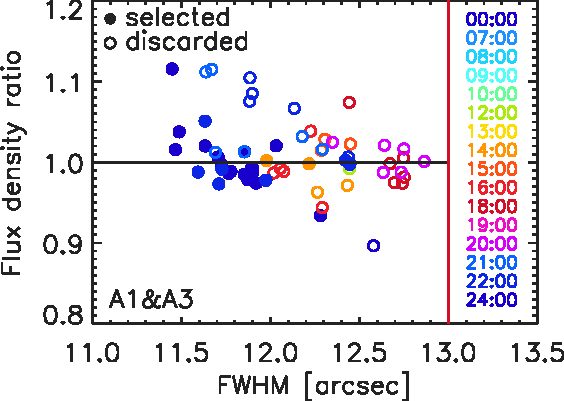
\includegraphics[clip=true, trim={0, -0.3cm, -0.3cm, 0}, width=0.35\textwidth]{Figures/Calibration/plot_flux_density_ratio_fwhm_uranus_corrected_skydip_narrow_1mm.pdf}
    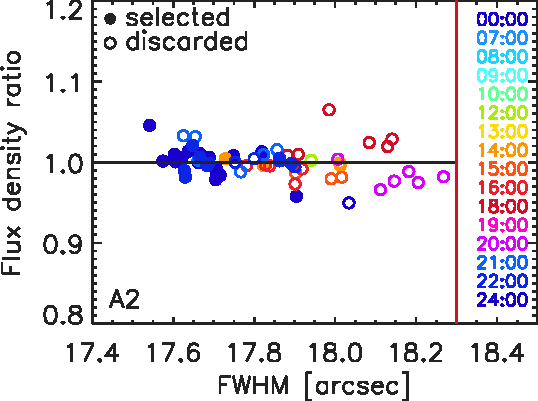
\includegraphics[clip=true, trim={0, -0.3cm, -0.3cm, 0}, width=0.3337\textwidth]{Figures/Calibration/plot_flux_density_ratio_fwhm_uranus_corrected_skydip_narrow_a2.pdf}
    % taumeter
    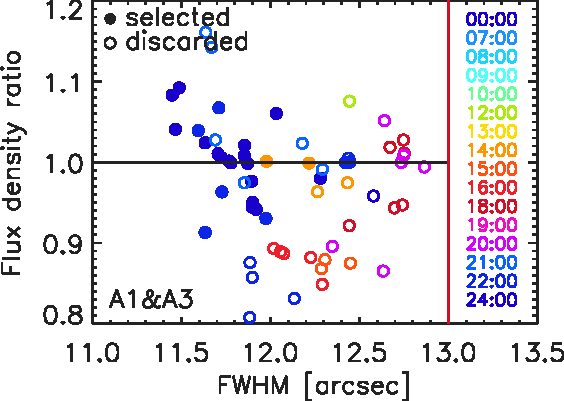
\includegraphics[clip=true, trim={0, -0.3cm, -0.3cm, 0}, width=0.35\textwidth]{Figures/Calibration/plot_flux_density_ratio_fwhm_uranus_tau225_narrow_1mm.pdf}
    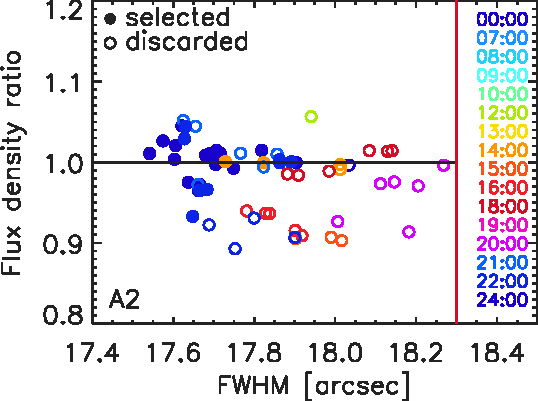
\includegraphics[clip=true, trim={0, -0.3cm, -0.3cm, 0}, width=0.3337\textwidth]{Figures/Calibration/plot_flux_density_ratio_fwhm_uranus_tau225_narrow_a2.pdf}
    % skydip
    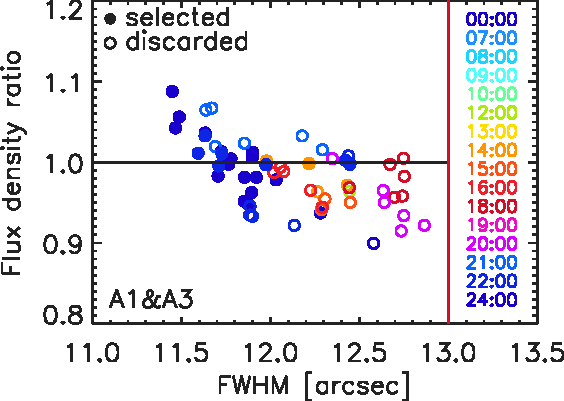
\includegraphics[clip=true, trim={0, -0.3cm, -0.3cm, 0}, width=0.35\textwidth]{Figures/Calibration/plot_flux_density_ratio_fwhm_uranus_skydip_narrow_1mm.pdf}
    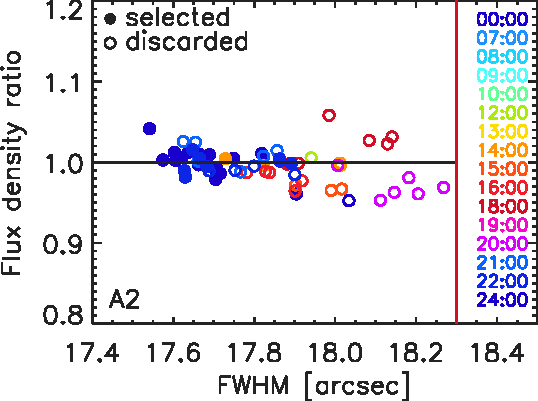
\includegraphics[clip=true, trim={0, -0.3cm, -0.3cm, 0}, width=0.3337\textwidth]{Figures/Calibration/plot_flux_density_ratio_fwhm_uranus_skydip_narrow_a2.pdf}
    % corr. sky. photocorr demo
    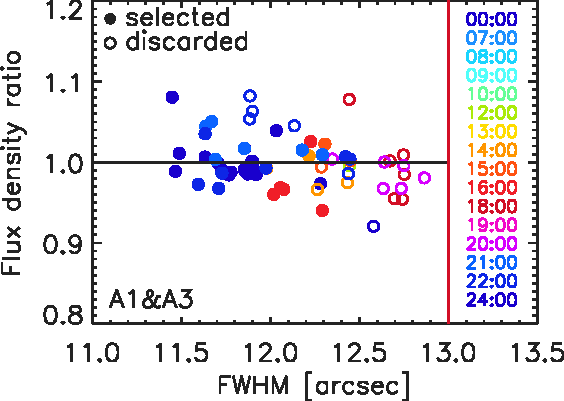
\includegraphics[clip=true, trim={0, -0.3cm, -0.3cm, 0}, width=0.35\textwidth]{Figures/Calibration/plot_flux_density_ratio_fwhm_uranus_corrected_skydip_photocorr_demo_narrow_1mm.pdf}
    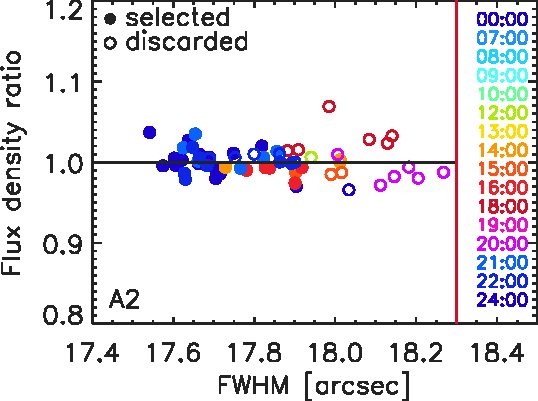
\includegraphics[clip=true, trim={0, -0.3cm, -0.3cm, 0}, width=0.3337\textwidth]{Figures/Calibration/plot_flux_density_ratio_fwhm_uranus_corrected_skydip_photocorr_demo_narrow_a2.pdf}
    % corr. sky. photocorr pointing
    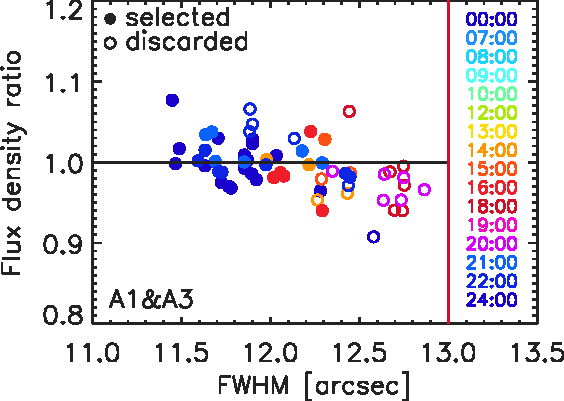
\includegraphics[clip=true, trim={0, -0.3cm, -0.3cm, 0}, width=0.35\textwidth]{Figures/Calibration/plot_flux_density_ratio_fwhm_uranus_corrected_skydip_photocorr_pointing_narrow_1mm.pdf}
    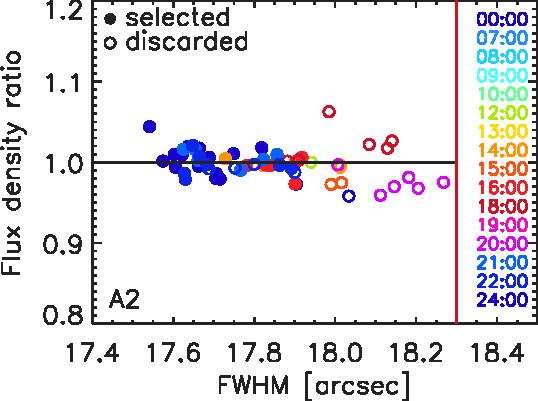
\includegraphics[clip=true, trim={0, -0.3cm, -0.3cm, 0}, width=0.3337\textwidth]{Figures/Calibration/plot_flux_density_ratio_fwhm_uranus_corrected_skydip_photocorr_pointing_narrow_a2.pdf}
    \caption[Uranus flux density stability against FWHM]{
      Uranus flux density ratio vs beam size for five
      calibration methods. The ratio of 
      Uranus measured flux densities to expectations in fonction of the
      measured 2D Gaussian beam FWHM is shown for the $1$-mm array
      combination (left column) and for array 2 (right column) after absolute
      calibration using (\emph{first row}:) the baseline method, as
      well as (\emph{second row}:) the 'taumeter'-based and
      (\emph{third row}:) the 'skydip'-based methods, and methods
      relying to (\emph{fourth row}:) the 'demo' and (\emph{fifth
        row}:) the 'pointing' photometric corrections. These plots
      include all Uranus scans acquired during N2R9, N2R12 and N2R14
      campaigns and whose beam FWHM are below the threshold indicated
      by the vertical red lines, (open circles), as
      well as the scans that met the baseline selection criteria (filled
      circles).}
\label{fig:calib_uranus_vs_fwhm_all}
\end{center}
\end{figure}


\subsection{Stability against the observed opacity}

\addparag{ stability against opacity}

\begin{figure}[ht!]
  \begin{center}
    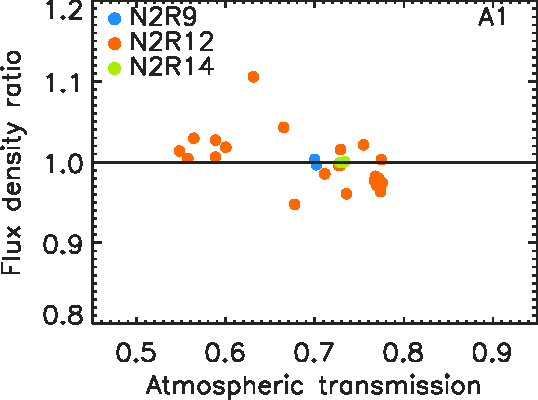
\includegraphics[clip=true, trim={0, -0.3cm, -0.3cm, 0}, width=0.35\textwidth]{Figures/Calibration/plot_flux_density_ratio_obstau_uranus_corrected_skydip_narrow_a1.pdf}
    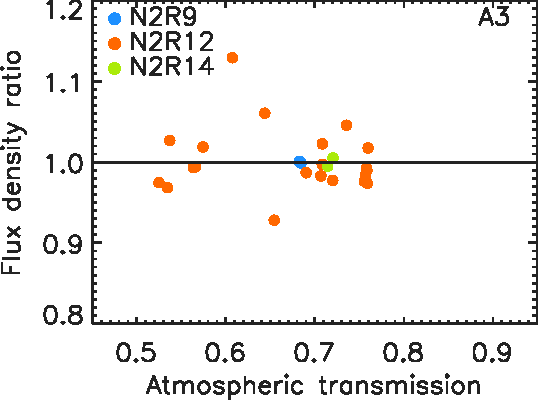
\includegraphics[clip=true, trim={0, -0.3cm, -0.3cm, 0}, width=0.35\textwidth]{Figures/Calibration/plot_flux_density_ratio_obstau_uranus_corrected_skydip_narrow_a3.pdf}
    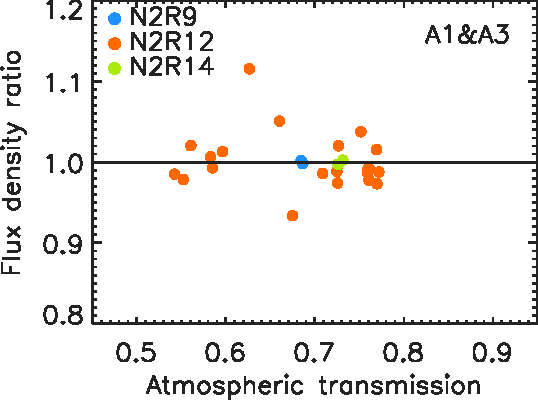
\includegraphics[clip=true, trim={0, -0.3cm, -0.3cm, 0}, width=0.35\textwidth]{Figures/Calibration/plot_flux_density_ratio_obstau_uranus_corrected_skydip_narrow_1mm.pdf}
    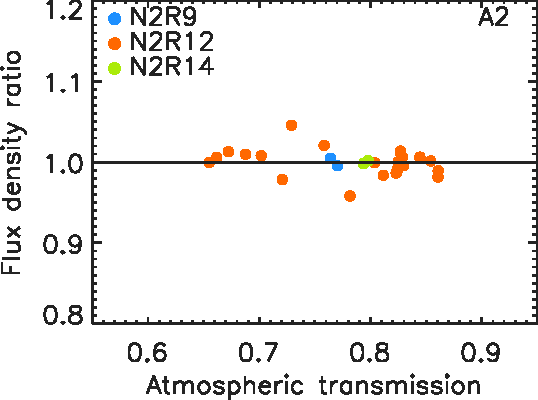
\includegraphics[clip=true, trim={0, -0.3cm, -0.3cm, 0}, width=0.35\textwidth]{Figures/Calibration/plot_flux_density_ratio_obstau_uranus_corrected_skydip_narrow_a2.pdf}
    \caption[Uranus flux density stability against observed
  opacity]{Uranus measured-to-modeled flux density ratio as a fonction
  of the measured observed opacity for array 1 (upper left), array 3
  (upper right), 1mm array combination (lower left) and array 2 (lower
  right). The datapoints denote the flux ratio of the scans retained after the
  baseline section is performed, for the three campaigns, N2R9
  in blue, N2R12 in orange and N2R14 in chartreuse (yellow green). For
  each campaign, flux ratios are equal to unity in average by
  construction and are stable againts the observed opacity, modelled as
  the zenith opacity times the air mass at the telescope elevation.}
\label{fig:uranus_flux_obstau}
\end{center}
\end{figure}
